%\lipsum[4-4]
In this chapter there are presented the future steps in research on outliers detection on railways WSN-based smart grid.


%%%%%%%%%%%%%%%%%%%%%
%%   Smart metering Systems
%%%%%%%%%%%%%%%%%%%%%
\section{Evaluation of effect of undetected outliers in railway WSN}


During the state of the art, the definition of "what is an outlier in railways WSN" was slightly covered, resulting in raising the research question: \textbf{What is the effect of an undetected outlier in railways WSN?}

A railways WSN is focused on acquiring the data (in forms of measurements) from the railways environment with the purpose of providing that information to a subsystem (such as a decision support system). Having this in mind, an assumption should be made to define the outlier as the effect of erroneous information retrieved from the DSS due to erroneous data from the measurement. A major contribution of an outlier detection mechanism is the validation of the quality of the output of the DSS. In particular, if a measurement or a set of measurements are detected as outliers, the DSS will have the information of the quality of his output, as is shown in figure \ref{fig:evaluation}.

\begin{figure}[h!]
	\centering
	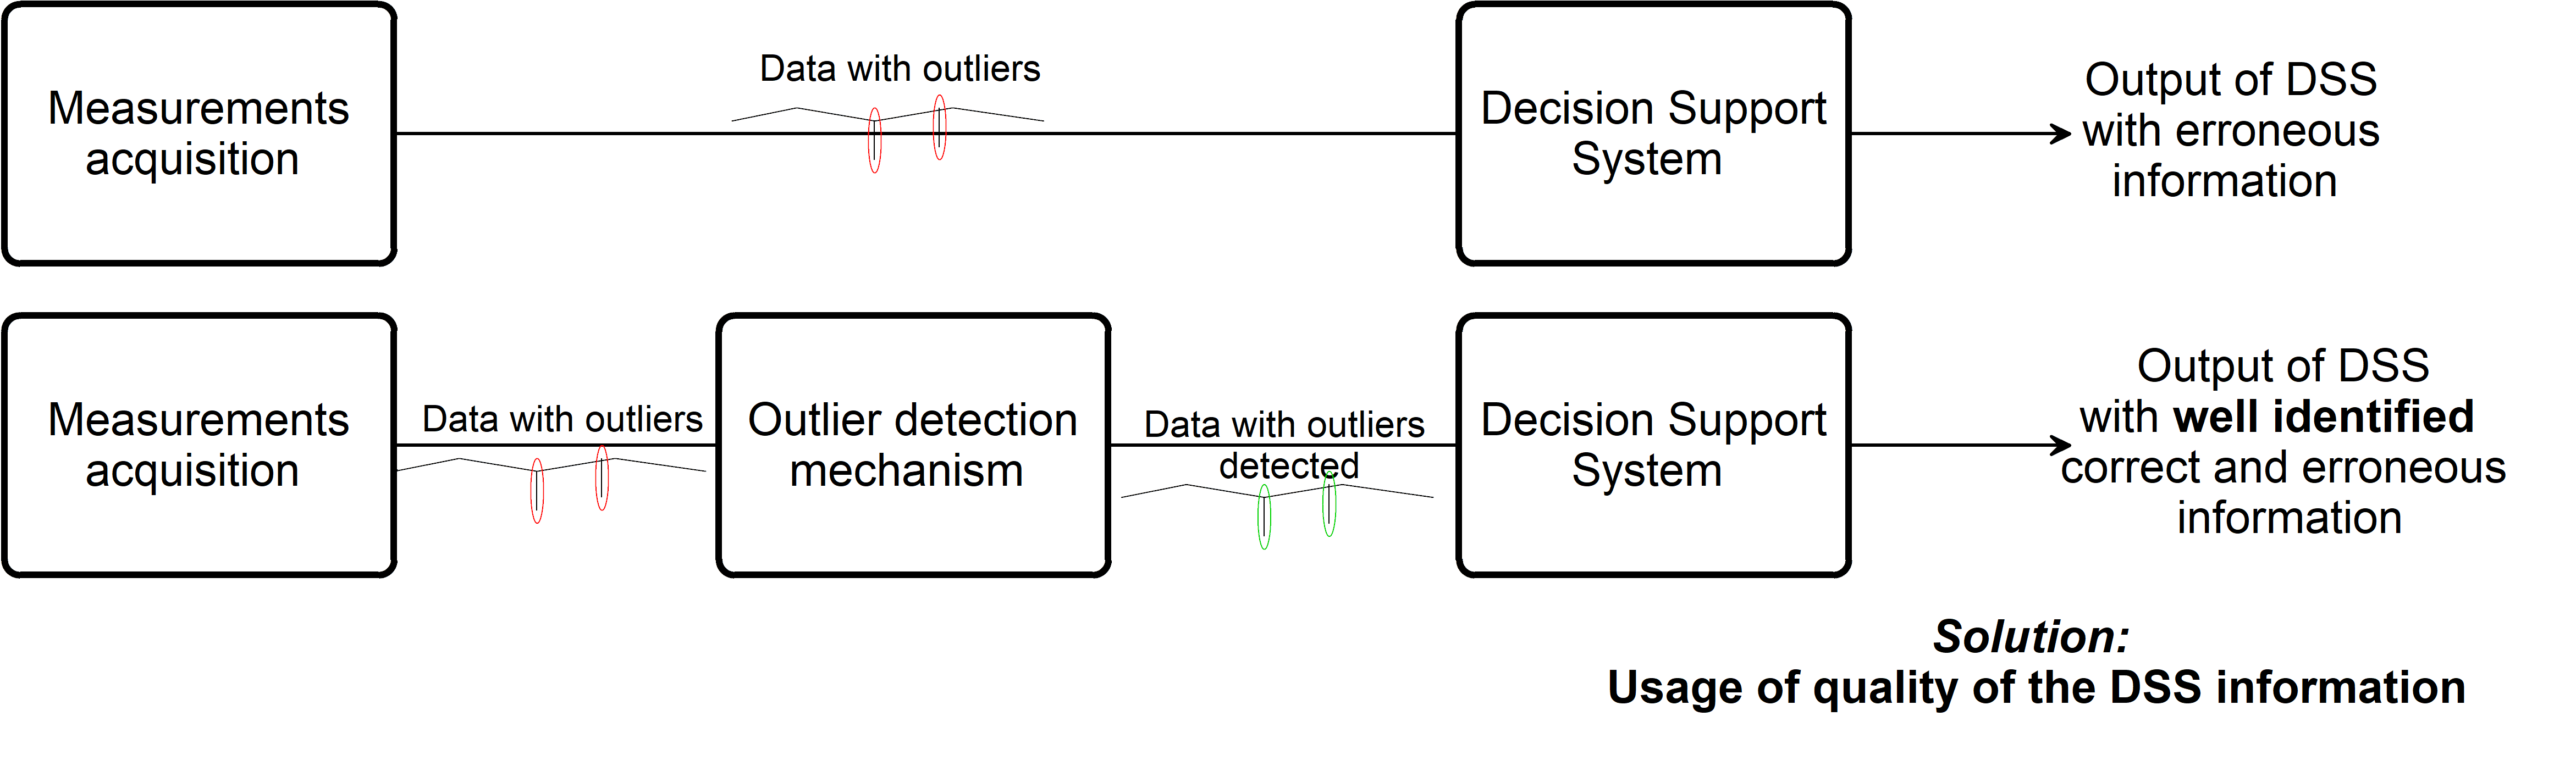
\includegraphics[width=1.03\textwidth,keepaspectratio]{figures/evaluation}
	\caption{Comparison of the output of DSS with and without an outlier detection mechanism. }
	\label{fig:evaluation}
\end{figure}

It is important at this moment to present examples of DSS. Eco-driving strategies and timetable planning require conservative measurements of energy consumption in several points of the railway electrical system, where the situations of outliers should result, in example, in default outputs of DSS; On other side, preventive maintenance may find resourceful the presence of outliers considering that those outliers reflect anomalous behavior due to unknown external effects (on the measurement).


The methodology will embrace the simulation of the railway WSN system. With a well defined simulation model that mimics the behavior of


\section{Selection of Outlier detection mechan}

\lipsum[1]
